% !TeX root = ../main.tex
% %%%%%%%%%%%%%%%%%%%%%%%%%%%%%%%%%%%%%%%%%%%%%%%%%%%%%%%%%%%%%%%%%%%%%%%%%%%%%%
% Introduction
\chapter{Introduction}
\label{chap:introduction}

Robotics already have a great impact in our current society so, 
the quality of software used by robots should be of extreme importance for us.
Robot software as well as the techniques used to test their quality are 
very specific to the field and differ a lot from the norm.
Automatic tests are barely used in robotics due to multiple factors.
The intention is then to create a tool that will promote the safe 
and reliable execution of automatic tests.
This tool will contemplate both a descriptive high-level language 
that should capture certain properties of a robot and a way to create test scenarios.

% ------------------------------------------------------------------------------
% Motivation
\section{Motivation}
\label{sec:motivation}

Currently, robots are vastly used industrially (medicine, agriculture, etc.) 
or as a form of leisure (contests, personal use, etc.).
The tendency is for robot usage to keep growing at a global level.
Robot tasks tend to be repetitive and/or rather specific.
Robot software also tends to be quite different from conventional software.
The Cyber-Physical systems of robots are non-deterministic and unreliable.
One reason is the fact that robots interact directly with their environment.
A sensor can return imprecise values since the environment itself can be very hard to predict.
As a result, the notion that a task or movement is correct is really hard for a robot to conceive.

\par

\alcides{Falas em testes automáticos, mas deverias primeiro identificar soluções para evitar isto. Introduzir primeiro testes, depois testes automáticos.}

Consequentemente testes 
automáticos são difíceis de realizar nesta área, de facto atualmente a grande maioria dos testes 
realizados em robôs necessitam de supervisionamento humano seja o teste feito no mundo real ou numa 
simulação, identifica-se assim que existe um espaço para melhoramento na área de testes para robôs 
através de testes automáticos optimizados com o objectivo de melhorar a qualidade destes sistemas.

\section{Problem Statement}
\label{sec:problem}

There are multiple challenges in robot testing, costs, 
complexity, hardware integration, among others.
When planning on how to test a robot there are tradeoffs between the 
different choices to make given into account all the challenges.
While tests using simulations are a promising approach for automation 
there is still distrust in the precision and validity of the results.
This means, although dangerous and sometimes expensive real-life 
robot testing is still the prime choice.
Be the tests done in the real world or resorting to simulation, 
human supervising will most likely still be necessary.
This is because identifying if a robot fulfills an expected 
behavior is really hard for the robot itself.
For this reason, automatic tests in the robotics field are 
hardly reliable and hard to implement.
The resulting product is a lack of quality in the software across projects~\cite{TestRob}.

% ------------------------------------------------------------------------------
% Objectives
\section{Objectives}
\label{sec:objectives}

This work has the objective of showing the potencial of automatic 
tests in robotics and of simplifying their execution.
With this in mind, the proposal is to create a mechanism that can be able 
to monitor certain components of the robot during or after a test execution.
These components aren't arbitrary but defined by the help of a descriptive high-level language.
The objective of the language is to describe a robot property in a simple and intuitive way.
This language will need to be supported by a compiler. 
The compiler should translate the language to a monitoring mechanism.
In this way, if a robot doesn't follow the properties defined by the language 
during a test, the compiler will infer that the robot behavior isn't correct.

\par

The Robot Operating System (ROS) is a collection of libraries and tools that help 
build robot software. ROS is the most widely used tool for writing robot software.
Robot simulation is an essential tool for testing. Gazebo offers the ability 
to simulate populations of robots in complex environments.
This being said, the final scheme of the tool that will accomplish the objective 
should look something like the below image.

\begin{figure}[h!]
    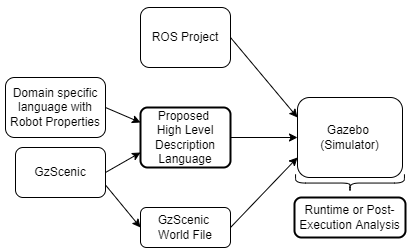
\includegraphics{images/intro_diag.png}
    \caption{Tool for monitoring robot properties.}
    \label{fig:intro_objectives}
\end{figure}

\section{Contributions}
\label{sec:contributions}

The expected contributions of this thesis are below enumerated.

\begin{enumerate}
    \item Definition of a descriptive high-level language to specify robots properties.
    \item A compiler for the language that can be used for monitoring.
    \item After evaluating the capability of the solution. Model multiple relevant problems in robotics.
\end{enumerate}

% ------------------------------------------------------------------------------
% Structure of the document
\section{Structure of the document}
\label{sec:structure}

The document is organized as follows:

\begin{itemize}
    \item Section 1...
    \item Section 2...
    \item Section 3...
\end{itemize}

